\chapter{Конструкторский раздел}
\label{cha:design}

\section{Требования к разрабатываемому программному обеспечению}
К разрабатываемому программному обеспечению предъявляются следующие высокоурованевые требования:
\begin{itemize}
 \item разрабатываемое программное обеспечение должно обеспечивать функционирование по требованию пользователя,
 \item программное обеспечение должно производить кодирование и декодирование указанного файла с графическими данными,
 \item программное обеспечение должно проводить анализ графических данных и осуществлять разбиение графических данных на блоки,
 \item программное обеспечение должно выполнять прямое и обратное вейвлетное преобразование блоков графических данных,
 \item программное обеспечение должно выполнять децимацию графических данных после применения вейвлетного преобразования.
\end{itemize}

\section{Пользовательские требования к программному обеспечению}
Пользовательские требования (функциональные требования с точки зрения пользователей) описывают цели и задачи пользователей
программного обеспечения, которые должны достигаться и выполняться пользователями при помощи разрабатываемого программного обеспечения.
К разрабатываемому программному обеспечению предъявляются следующие требования:
\begin{itemize}
 \item разрабатываемое программное обеспечение должно позволять пользователю выбирать файл с графическими данными,
 \item программное обеспечение должно позволять пользователю задавать процент сохраняемых данных,
 \item программное обеспечение должно позволять пользователю выполнять кодирование файла с графическими данными с помощью разработанного метода 
 с использованием кратномасштабного анализа,
 \item программное обеспечение должно позволять пользователю выполнять декодирование файла с преобразованными графическими данными,
 \item программное обеспечение должно выполнить воспроизведение графических данных после декодирования.
\end{itemize}

\section{Входные и выходные параметры}
Разрабатываемое программное обеспечение состоит из двух частей:
\begin{itemize}
 \item кодирование графических данных,
 \item декодирование графических данных.
\end{itemize}
Входными данными для функционала кодирования графических данных являются исходный файл с графическими даннными и процент сохраняемых данных.
Выходными данными для функционала кодирования графических данных является файл, содержащий кодированную последовательность графических данных после
применения вейвлетного преобразования и децимации.
Входными данными для функционала декодирования графических данных являются исходный файл с кодированными графическими даннными.
Выходными данными для функционала декодирования графических данных является последовательность кадров, состоящая из графических данных, полученных после применения 
обратного вейвлетного преобразования.

\section{Сценарии функционирования}
Сценарии функционирования разрабатываемого программного комплекса представлены на рисунке \ref{fig:uml1}.

\begin{figure}[ht]
  \centering
  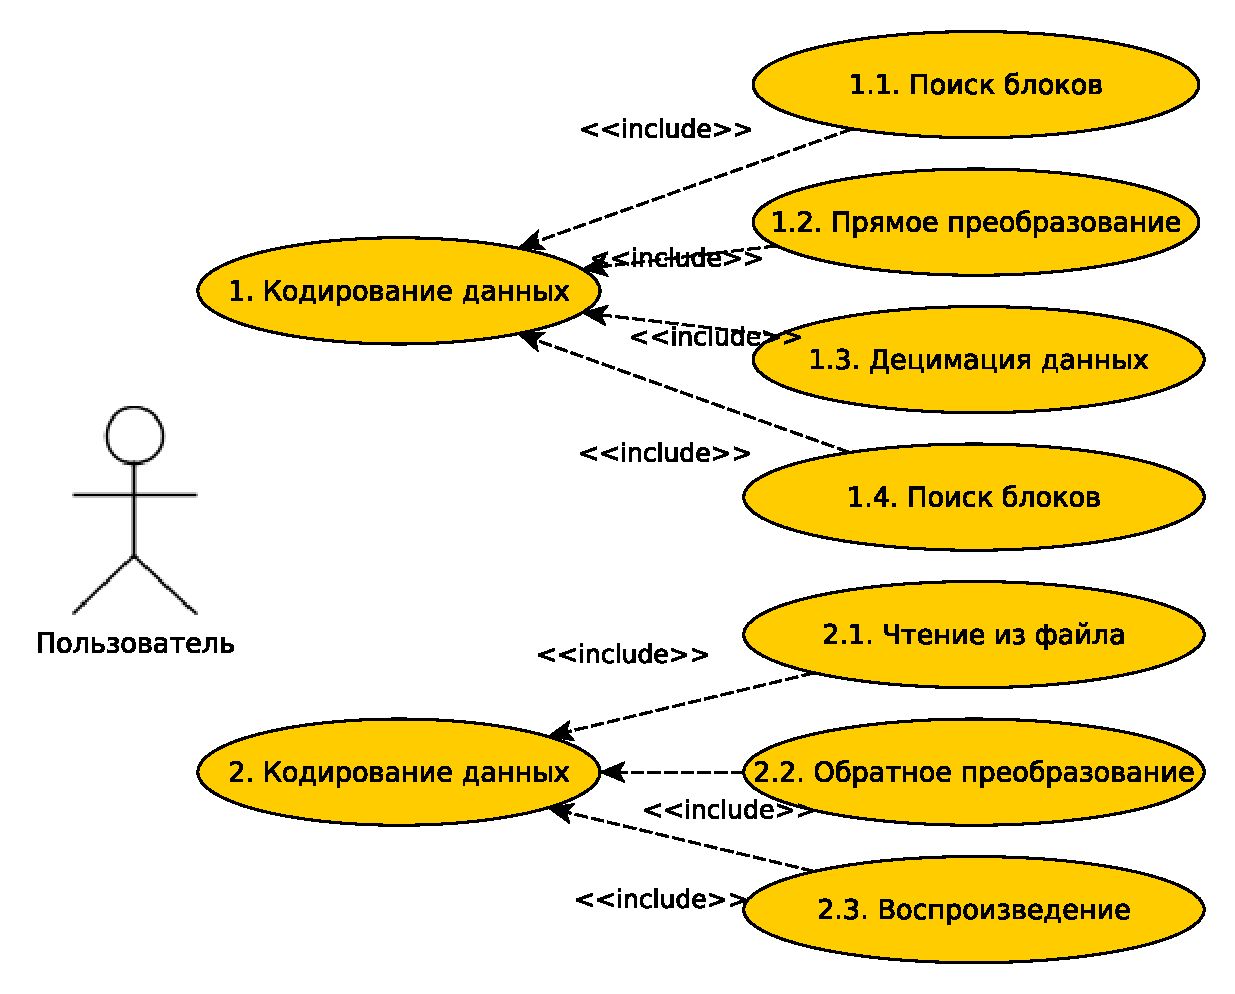
\includegraphics[scale=0.65]{inc/graphics/uml1.pdf}
  \caption{Диаграмма вариантов использования с точки зрения пользователя}
  \label{fig:uml1}
\end{figure}

Возможны следующие сценарии использования программного обеспечения:
\begin{itemize}
 \item Прецедент 1 - Кодировать данные
    \subitem Прецедент 1.1 - Анализ графических данных и поиск блоков
    \subitem Прецедент 1.2 - Прямое вейвлетное преобразование
    \subitem Прецедент 1.3 - Децимация графических данных
    \subitem Прецедент 1.4 - Запись кодированных данных в файл
 \item Прецедент 2 - Декодировать данные
    \subitem Прецедент 2.1 - Чтение графических данных из файла
    \subitem Прецедент 2.2 - Обратное вейвлетное преобразование
    \subitem Прецедент 2.3 - Воспроизведение видео
\end{itemize}



\section{Алгоритм сжатия видео с использованием кратномасштабного анализа}
В соответствии со схемой \ref{fig:figalg} прямого и обратного преобразования был разработан алгоритм сжатия видео.

В разрабатываемой системе важна скорость сжатия. Поэтому для разбиения на блоки использовалась 
усредненная абсолютная разность значений цветовых компонент, так как для ее определения необходимо наименьшее количество вычислений.

Для вейвлетного преобразования необходимо выделить параметры, которые влияют на поведение системы.
Были выделены следующие параметры:
\begin{itemize}
 \item Размер блока
 \item Порядок системы коэффициентов для вейвлетного преобразования
 \item Процент сохраняемых данных
 \item Алгоритм кодирования без потерь
\end{itemize}
Эти параметры передаются как входные данные вместе с графическими данными.

В разрабатываемой системе для выполнения вейвлет-преобразования необходимо разработать отдельный модуль. 
Для прямого и обратного преобразований необходимо получить систему вейвлет-коэффициентов нужного порядка. 
Для этого необходимо разработать функции получения набора коэффициентов указанной системы коэффициентов. 

Для алгоритма прямого преобразования необходимо инициализировать размер рассматриваемой области. 
В начале работы алгоритма размер рассматриваемой области равен размеру блока. 
В процессе работы алгоритма размер рассматриваемой области уменьшается. 
Если ширина, высота, глубина рассматриваемой области равны единице, то необходимо закончить вейвлет-преобразование. 

На каждой итерации вейвлет-преобразование применяется ко всем векторам рассматриваемой области 
блока сначала по ширине, затем по высоте, затем по глубине, ширина, высота и глубина рассматриваемой области уменьшаются в два раза. 
Для выполнения вейвлет-преобразования необходимо составить матрицу вейвлет-преобразования в соответствии с 
размером рассматриваемой области. 
Прямое вейвлет-преобразование может быть реализовано как рекурсивно, так и итеративно. 
Подробная схема разработанного алгоритма прямого вейвлет-преобразования представлена на рисунке \ref{fig:figalgdir}. 
Код процедуры прямого вейвлетного преобразования блока представлен в листинге \ref{lst:dir}, где \texttt{block} - графические данные, которые необходимо преобразовать,
\texttt{block\_size} - количество кадров в блоке, \texttt{с} - количество каналов в блоке, \texttt{h} - высота блока, \texttt{w}
- ширина блока, \texttt{s} - система коэффициентов, \texttt{p} - процент 
сохраняемых данных.

\begin{figure}
  \centering
% [width=0.5\textwidth] --- регулировка ширины картинки
  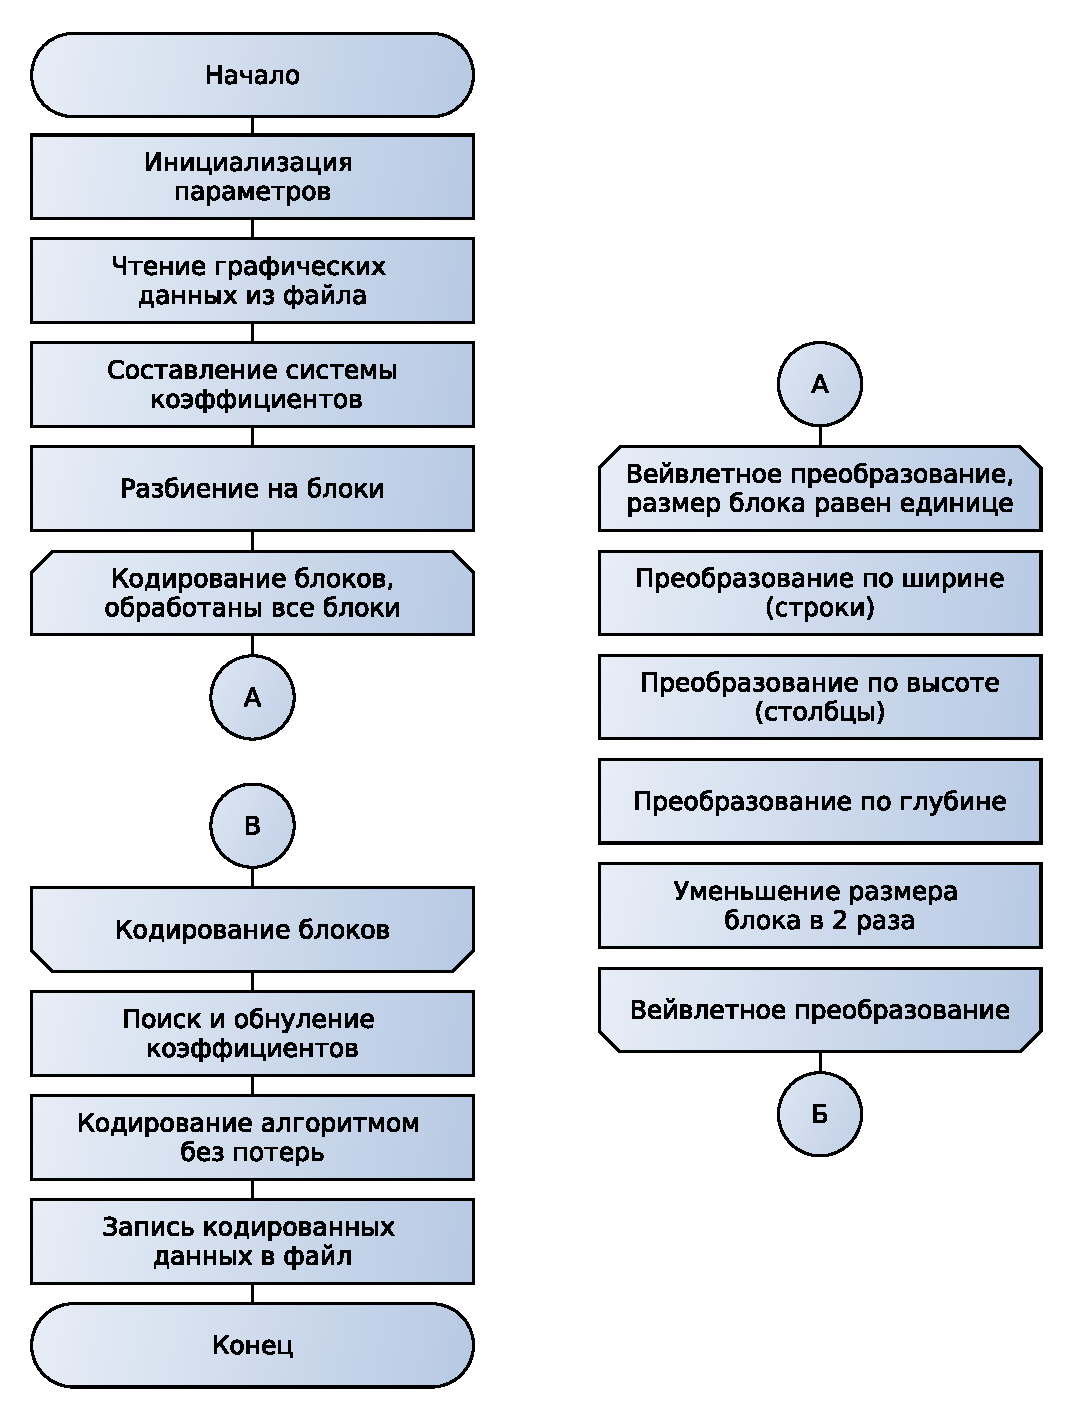
\includegraphics[scale=0.75]{inc/graphics/alg1.pdf}
  \caption{Cхема компрессии видео}
  \label{fig:figalgdir}
\end{figure}

\begin{lstlisting}[style=pseudocode,caption={Код процедуры transform\_block},label=lst:dir]
transform_block(block, block_size, c, h, w, s, p)
  block_data := CopyBlockData(block, block_size, c, h, w)
  DirectTransform(block_data, c, w, h, block_size, w, h, block_size, s)
  out_data := Decimate(block_data, c, w, h, block_size, p)
  FreeBlockData(block_data, block_size, c, h, w)
  return out_data
\end{lstlisting}
   
Для алгоритма обратного преобразования необходимо рассчитать размер рассматриваемой области, 
так как блок может иметь разные размеры по высоте, ширине и глубине. В процессе работы алгоритма 
размер рассматриваемой области увеличивается. Если ширина и высота рассматриваемой области 
соответствуют размерам изображения, то необходимо закончить обратное вейвлет-преобразование.
Подробная схема разработанного алгоритма обратного вейвлет-преобразования представлена на рисунке \ref{fig:figalg2}.
Код процедуры обратного вейвлетного преобразования блока представлен в листинге \ref{lst:back}, где \texttt{out\_data} - кодированные данные, к которым 
необходимо применить обратное вейвлетное преобразование,
\texttt{block\_size} - количество кадров в блоке, \texttt{с} - количество каналов в блоке, \texttt{h} - высота блока, \texttt{w}
- ширина блока, \texttt{s} - система коэффициентов

\begin{lstlisting}[style=pseudocode,caption={Код процедуры decode\_block},label=lst:back]
decode_block(out_data, block_size, c, h, w, system)
  block_data = AllocateBlock(block_size, c, h, w)
  ConvertArrayToMatrix(out_data, block_data)
  InverseTransform(block_data, c, w, h, block_size, w, h, block_size, system)
  block = AllocateFrames(block_size, c, h, w)
  for int i := 0; i < block_size; ++i
    block[i] = WriteImageData(block_data[i])
  FreeBlockData(block_data, block_size, c, h, w)
  return block
\end{lstlisting}


\begin{figure}
  \centering
  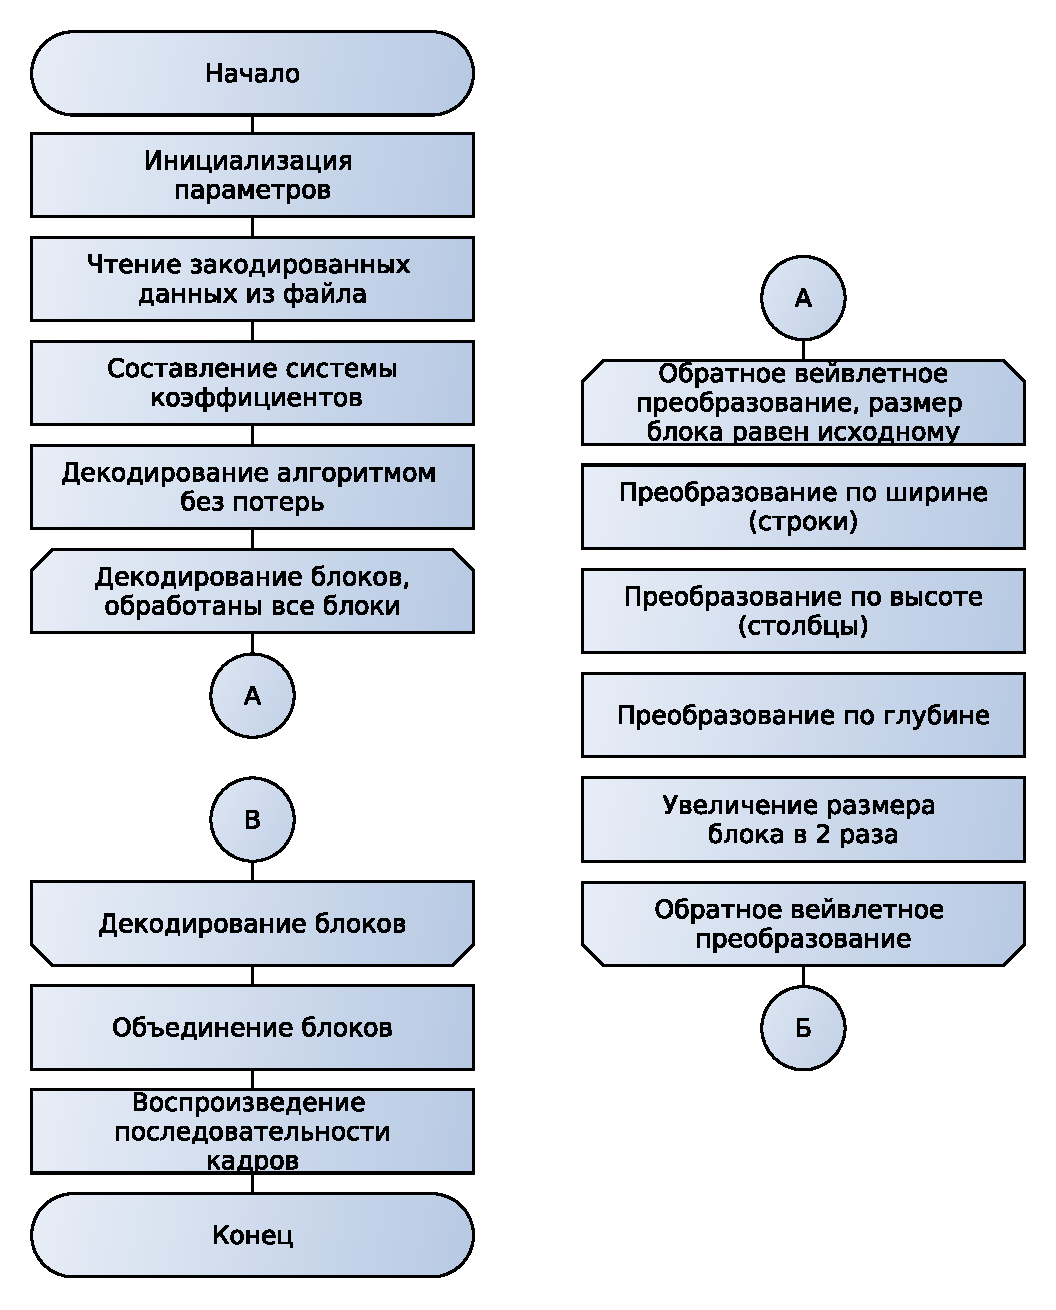
\includegraphics[scale=0.75]{inc/graphics/alg2.pdf}
  \caption{Cхема компрессии видео}
  \label{fig:figalg2}
\end{figure}


\section{Составление матриц}
В данной работе для рассмотрения выбраны вейвлеты Добеши, так как предполагается, 
что увеличение размера системы коэффициентов приводит к лучшей сжимаемости \cite{Pup01}.
Матрица прямого преобразования M состоит из двух прямоугольных матриц L и H,  
представляющих низкочастотный и высокочастотный фильтры. Матрицы L и H могут быть составлены следующим образом:
\begin{equation}
L= \begin{cases}
 c_{j-2i+1+n}, \mbox{при $j-2i+1<0$} \\
 c_{j - 2i + 1}, \mbox{иначе}
\end{cases}
\label{F:F2}
\end{equation}
\begin{equation}
L= \begin{cases}
 (-1)^{j+1}c_{2i-j+n}, \mbox{при $2i-j<0$} \\
 (-1)^{j+1}c_{2i-j}, \mbox{иначе}
\end{cases}
\label{F:F2}
\end{equation}              
Матрица обратного преобразования является транспонированной матрицей прямого преобразования. Код процедуры заполнения 
матрицы преобразования представлен в листинге \ref{lst:PrepareMatrix}, где m - матрица преобразования, dim - размерность матрицы
преобразования, system - выбранная система коэффициентов.
        
\begin{lstlisting}[style=pseudocode,caption={Код процедуры PrepareMatrix},label=lst:PrepareMatrix]
PrepareMatrix(m, dim, system)
  if dim % 2 != 0
    then dim := dim - 1
  i := 0
  j := 0
  for i := 0; i < dim / 2; ++i
    for j := 0; j < dim; ++j)
      index := (j + 1) - 2 * (i + 1) + 1
      system_index := index < 0 ? index + dimension : index
      m[i][j] := system_index >= 0 && system_index < system.size ? system[system_index] : 0
      
  for i := 0; i < dim / 2; ++i)
    for j := 0; j < dim; ++j
      index := 2 * (i + 1) - (j + 1);
      system_index := index < 0 ? index + dimension : index
      if system_index < 0 or system_index >= system.size()
        then m[i + dim / 2][j] := 0
        else
          if (j + 2) % 2 != 0
            then m[i + dim / 2][j] = -system[system_index]
            else m[i + dim / 2][j] = system[system_index]
\end{lstlisting}

\section{Поиск и обнуление минимальных коэффициентов после применения вейвлет-преобразования}
После применения прямого вейвлетного преобразования необходимо обеспечить 
сжатие путем обнуления части коэффициентов. Степень сжатия задается 
пользователем в процентах. Из ненулевых элементов необходимо выбрать указанный пользователем процент 
максимальных элементов. Это значит, что необходимо найти указанную пользователем 
порядковую статистику в наборе графических данных. 
Видео содержит большое количество кадров, каждый кадр содержит несколько каналов, 
массив графических данных может содержать по несколько тысяч элементов. 
Поэтому необходимо производить эффективный поиск порядковой статистики. Рассмотрим 
алгоритм, выполняющий поиск порядковой статистики за линейное время $O(n)$, где $n$ - 
размерность входных данных для поиска порядковой статистики.
Заранее не известно количество ненулевых элементов в массиве, 
для определения номера искомой порядковой статистики необходимо подсчитать количество ненулевых элементов. 
Зная это количество и указанный пользователем процент, точно определяется номер искомой порядковой статистики. 

Алгоритм \texttt{Randomized\_Select} поиска порядковой статистики разработан по аналогии 
с алгоритмом быстрой сортировки. Как и в алгоритме быстрой сортировки, в алгоритме 
\texttt{Randomized\_Select} используется идея рекурсивного разбиения входного массива. 
В отличие от алгоритма быстрой сортировки, в котором рекурсивно обрабатываются обе части разбиение, 
алгоритм \texttt{Randomized\_Select} работает лишь с одной частью. Это различие проявляется 
в результатах анализа обоих алгоритмов: если математическое ожидание времени работы
алгоритма быстрой сортировки равно $\Theta(n \lg n)$, то ожидаемое время работы алгоритма 
\texttt{Randomized\_Select} равно $\Theta(n)$, в предположении, что все элементы входных множеств различны.

В алгоритме \texttt{Randomized\_Select} используется процедура Randomized\_Partition. 
Подобно быстрой сортировке, \texttt{Randomized\_Select} – рандомозированный алгоритм, 
поскольку его поведение частично определяется выводом генератора случайных чисел. 
Код процедуры \texttt{Randomized\_Select} представлен в листинге \ref{lst:RandomizedSelect}, где входные параметры A – Массив данных,
p – левая граница части массива для поиска,
r – правая граница части массива для поиска,
i – номер искомой порядковой статистики, возвращаемое значение это искомая порядковая статистика.

        
\begin{lstlisting}[style=pseudocode,caption={Код процедуры Randomized\_Select},label=lst:RandomizedSelect]
Randomized_Select(A, p, r, i) 
  if p = r 
    then return A[p] 
  q := Randomized_Partition(A, p, r) 
  k := q - p + 1
  if i = k
    then return A[q]
  else if i < k
    then return Randomized_Select(A, p, q - 1, i)
  else return Randomized_Select(A, q + 1, r, i - k)
\end{lstlisting}
        
После выполнения процедуры \texttt{Randomized\_Partition}, которая вызывается  в строке 4 
представленного выше алгоритма, массив \texttt{А[р..r]} оказывается разбитым на два (возможно, пустых) 
подмассива \texttt{A[p..q-1]} и \texttt{A[q+l..r]}. При этом величина каждого элемента \texttt{A[p..q-1]} не превышает 
\texttt{A[q]}, а величина каждого элемента \texttt{А[q+1..r]} больше \texttt{A[q]}. 
Как и в алгоритме быстрой сортировки, элемент \texttt{A[q]} будем называть опорным (\texttt{pivot}). 
В строке 5 процедуры \texttt{Randomized\_Select} вычисляется количество элементов \texttt{k} подмассива \texttt{А[p..q]}, 
то есть количество элементов, попадающих в нижнюю часть разбиения плюс один опорный элемент. 
Затем в строке 6 проверяется, является ли элемент \texttt{A[q]} \texttt{i}-м в порядке возрастания элементом. 
Если это так, то возвращается элемент \texttt{A[q]}. В противном случае в алгоритме определяется, в 
каком из двух подмассивов содержится \texttt{i}-й в порядке возрастания элемент: в подмассиве \texttt{A[p..q-1]} 
или в подмассиве \texttt{A[q+l..r]}. Если \texttt{i < k}, то нужный элемент находится в нижней части разбиения, 
и он рекурсивно выбирается из соответствующего подмассива в строке 9. Если же \texttt{i > k}, то нужный элемент 
находится в верхней части разбиения. Поскольку уже известны \texttt{k} значений, которые меньше \texttt{i}-го в 
порядке возрастания элемента массива \texttt{А[р..г]} (это элементы подмассива \texttt{A[p..q]}), 
нужный элемент является \texttt{(i - k)}-м в порядке возрастания элементом подмассива \texttt{A[q + l..r]}, который рекурсивно находится в строке 10.
Опорный элемент выбирается в массиве случайным образом. Код процедуры \texttt{Randomized\_Partition} представлен в листинге \ref{lst:RandomizedPartition}, 
где входными параметрами являются A – массив данных, p – левая граница части массива для поиска, r – правая граница части массива для поиска,
возвращаемым значением является индекс опорного элемента.
 
\begin{lstlisting}[style=pseudocode,caption={Код процедуры Randomized\_Partition},label=lst:RandomizedPartition]
Randomized_Partition(A, p, r)
  i := Random( p, r )
  Swap( A[r], A[i] )
  return Partition( A, p, r )
\end{lstlisting}

Вместо того чтобы в качестве опорного элемента всегда использовать \texttt{А[r]}, 
такой элемент будет выбираться в массиве \texttt{A[p..r]} случайным образом. 
Процедура \texttt{Partition} выбора опорного элемента представлена в листинге \ref{lst:Partition}.

\begin{lstlisting}[style=pseudocode,caption={Код процедуры Partition},label=lst:Partition]
Partition(A, p, r)
  x := A[r] 
  i := p - 1
  for j := p to r - 1
    do if A[j] <= x
      then i := i + 1
        Swap( A[i], A[j] )
  Swap( A[i + 1], A[r] )      
  return i + 1
\end{lstlisting}

Рассмотренный алгоритм выполняет поиск порядковой статистики за линейное время \cite{Pup05}.

\section{Процессы, происходящие в разрабатываемой системе}
В разрабатываемой системе происходят следующие процессы:
\begin{itemize}
 \item чтение и запись графических данных в файл,
 \item операции выделения и освобождения памяти для вычислений,
 \item анализ графических данных для определения блоков,
 \item прямое и обратное вейвлет-преобразование данных,
 \item операции с матрицами для работы вейвлет-преобразования,
 \item состевление матрицы коэффициентов для вейвлет-преобразования,
 \item удаление части информации о видео после применения вейвлет-преобразования. 
\end{itemize}

В результате процессов, происходящих в разрабатываемой системе, 
была разработана схема основных модулей, необходимых для функционирования системы,       
представленная на рисунке \ref{fig:modules}. 

\begin{figure}
  \centering
  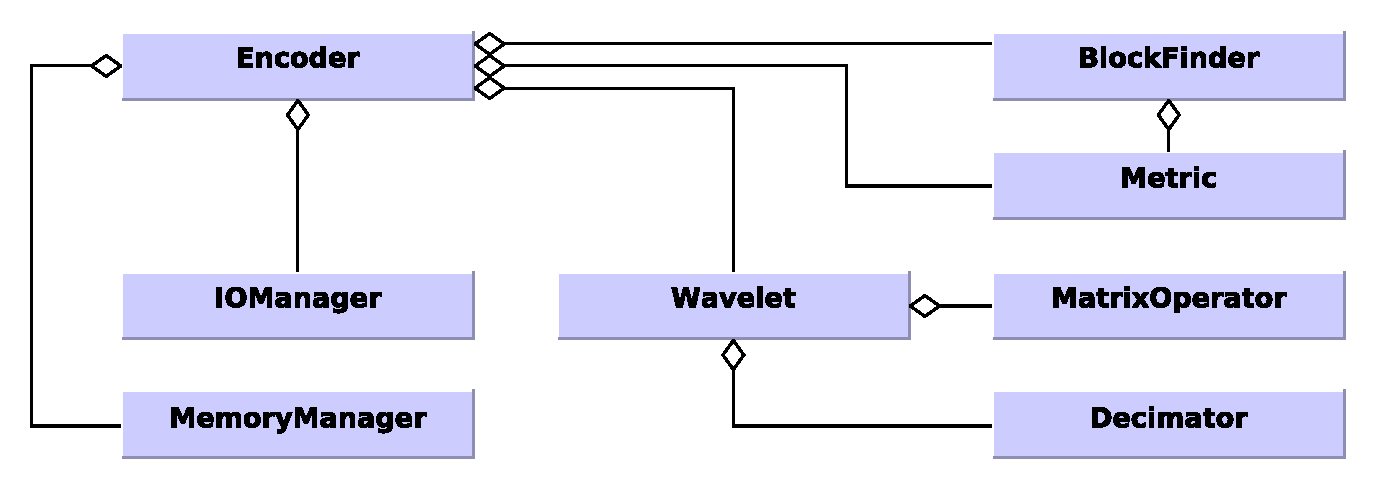
\includegraphics[scale=0.6]{inc/graphics/modules.pdf}
  \caption{Cхема модулей разрабатываемой системы}
  \label{fig:modules}
\end{figure}

Модуль \texttt{Encoder} является основным модулем разрабатываемой системы, в котором происходит весь процесс обработки 
графических данных от чтения графических данных из файла до записи закодированных графических данных в файл.
Содержит функции:

\begin{itemize}
 \item функция кодирования исходных графических данных,
 \item функция декодирования преобразованных графических данных.
\end{itemize}

Модуль \texttt{BlockFinder} вычисляет блоки, к которым будет применено вейвлетное преобразование. Содержит функцию
поиска блоков, принимающую на вход графические данные и возвращающую вычисленные блоки.

Модуль \texttt{IOManager} чтения/записи данных в файл при чтении получает от управляющего модуля имя файла и возвращает прочитанные графические данные, 
при записи получает от управляющего модуля имя файла и графические данные и возвращает результат выполнения операции записи. 
Содержит следующие функции:
\begin{itemize}
 \item функция чтения графических данных из файла,
 \item функция записи преобразованных графических данных в файл,
 \item функция чтения преобразованных графических данных из файла.
\end{itemize}

Модуль \texttt{MemoryManager} управляет памятью, необходимой для выполнения расчетов во время применения вейвлетного преобразования.
Содержит следующие функции:
\begin{itemize}
 \item функция выделения блока памяти для расчетов,
 \item функция освобождения выделенной памяти,
 \item функция копирования графических данных во временную память для применения прямого вейвлетного преобразования,
 \item функция копирования преобразованых данных во временную память для применения обратного вейвлетного преобразования.
\end{itemize}

Модуль вейвлетных преобразований \texttt{Wavelet} получает на вход графические данные и параметры преобразования, 
применяет к данным указанное преобразование, возвращает преобразованные данные. Содержит следующие функции:
\begin{itemize}
\item функция выполнения прямого вейвлетного преобразования,
\item функция выполнения обратного вейвлетного преобразования.
\end{itemize}

Для работы модуля вейвлетных преобразований требуется вспомогательный модуль работы с матрицами \texttt{MatrixOperator}, 
который производит умножение матрицы на вектор, а так же составление матриц для указанного вейвлетного преобразования. Содержит следующие функции:
\begin{itemize}
\item функция составления матрицы преобразования указанной размерности для указанной системы коэффициентов,
\item функция получения набора коэффициентов указанной системы коэффициентов,
\item функция умножения матрицы на вектор графических данных,
\item функция транспонирования матрицы.
\end{itemize}
Алгоритм составления матрицы представлен на рисунке 

Модуль выбора значимых коэффициентов \texttt{MatrixOperator} получает от модуля \texttt{Wavelet} графические данные и степень сжатия, 
удаляет указанную часть данных, возвращает обработанные данные. Содержит следующие функции: 
\begin{itemize}
\item функция удаления части графических данных,
\item функция поиска порядковой статистики.
\end{itemize}
